\documentclass{article}

\usepackage{graphicx}
\usepackage{amsmath}
\usepackage{fancyhdr}
\usepackage{float}
\usepackage{titlesec}
\usepackage{verbatim}
\usepackage{fancyvrb}
\usepackage[dvipsnames]{xcolor}
\usepackage[sorting=none]{biblatex}
\usepackage[margin=1in]{geometry}
\usepackage[font={small,it}]{caption}
\usepackage{placeins}
\usepackage{xepersian}


%%%%txt
\RecustomVerbatimCommand{\VerbatimInput}{VerbatimInput}%
{fontsize=\footnotesize,
 %
 frame=lines,  % top and bottom rule only
 framesep=2em, % separation between frame and text
 rulecolor=\color{Gray},
 %
 label=\fbox{\color{Black}txt file},
 labelposition=topline,
 %
 commandchars=\|\(\), % escape character and argument delimiters for
                      % commands within the verbatim
 commentchar=*        % comment character
}
%%%%txt


%\DeclareMathOperator*{\btie}{\bowtie}
\addbibresource{bibliography.bib}
\settextfont[Scale=1.2]{B-NAZANIN.TTF}
\setlatintextfont[Scale=1]{Times New Roman}
\renewcommand{\baselinestretch}{1.5}
\pagestyle{fancy}
\fancyhf{}
\rhead{تکلیف هفتم آزمایشگاه شبکه ‌های کامپیوتری}
\lhead{\thepage}
\rfoot{علیرضا ابره فروش}
\lfoot{9816603}
\renewcommand{\headrulewidth}{1pt}
\renewcommand{\footrulewidth}{1pt}

\begin{document}
\begin{titlepage}
\begin{center}

\includegraphics[width=0.4\textwidth]{figures/IUT Logo.png}\\
        
\LARGE
\textbf{دانشگاه صنعتی اصفهان}\\
\textbf{دانشکده مهندسی برق و کامپیوتر}\\
        
\vfill
        
\huge
\textbf{عنوان: تکلیف چهارم درس ریزپردازنده}\\
        
\vfill
        
\LARGE
\textbf{نام و نام خانوادگی: علیرضا ابره فروش}\\
\textbf{شماره دانشجویی: 9816603}\\
\textbf{نیم\,سال تحصیلی: پاییز 1400}\\
\textbf{مدرّس: دکتر عارف کریمی افشار}\\
\end{center}
\end{titlepage}


%\tableofcontents
\newpage



\section{}%1
ابتدا سناریو را به شکل زیر می‌بندیم و تجهیزات اولیه را به روترها اضافه می‌کنیم.
\begin{figure}[H]
    \centering
    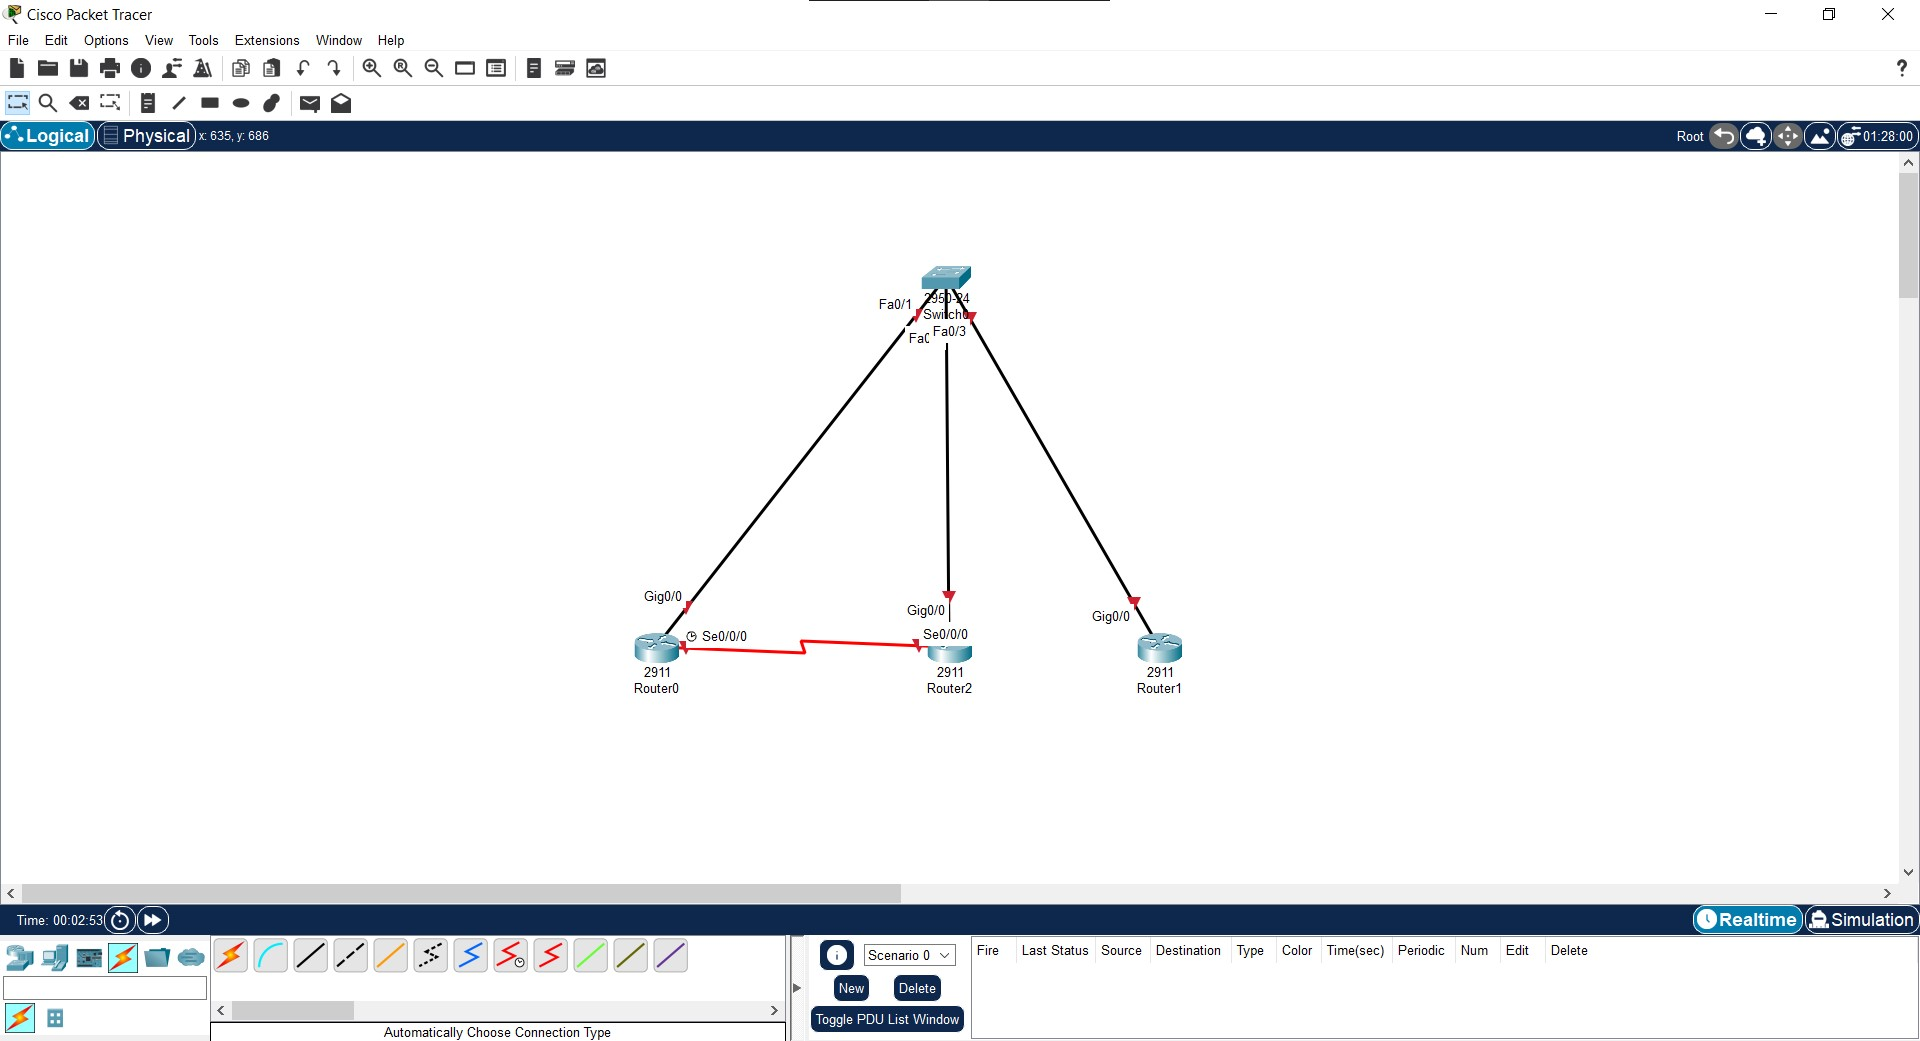
\includegraphics[width=1.0\textwidth]{figures/1.jpg}
    \caption{}
    \label{fig:fig1}
\end{figure}


\section{}%2
اینترفیس‌های \lr{fast} و \lr{serial} را به این طریق پیکربندی می‌کنیم.
\begin{figure}[H]
    \centering
    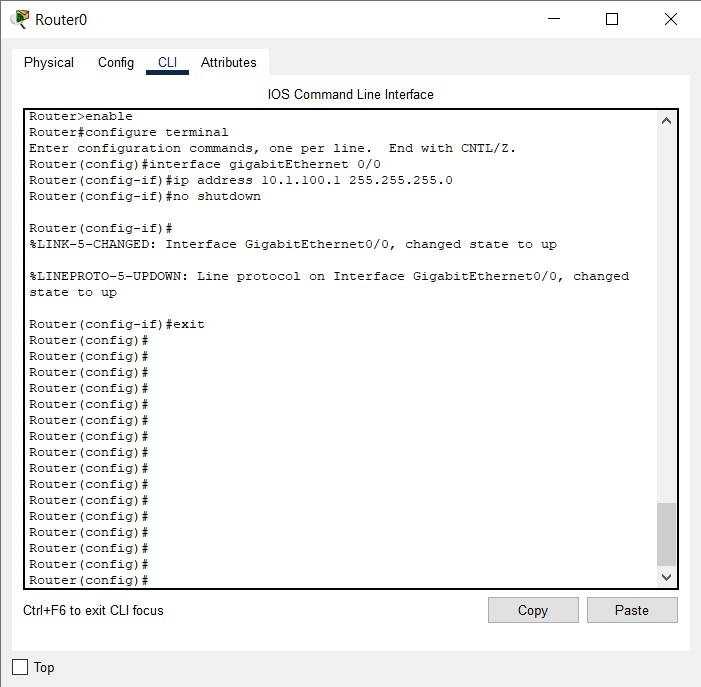
\includegraphics[width=0.75\textwidth]{figures/2.jpg}
    \caption{}
    \label{fig:fig1}
\end{figure}

\begin{figure}[H]
    \centering
    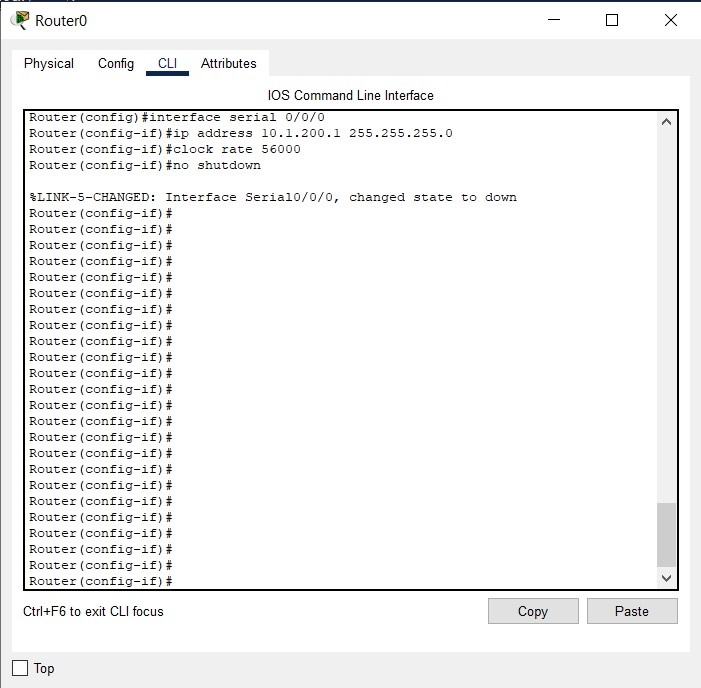
\includegraphics[width=0.75\textwidth]{figures/3.jpg}
    \caption{}
    \label{fig:fig1}
\end{figure}


\section{}%3
اینترفیس \lr{loopback} را به شکل زیر ایجاد می‌کنیم.
\begin{figure}[H]
    \centering
    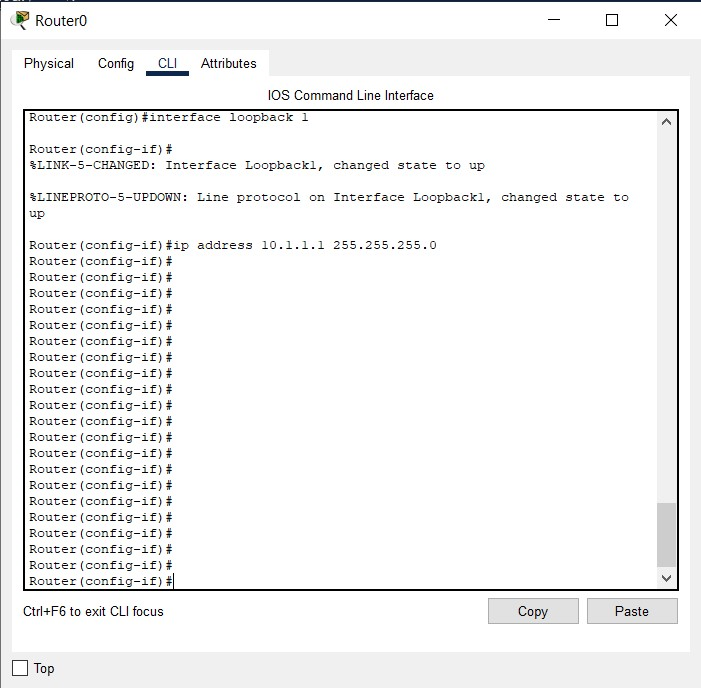
\includegraphics[width=0.75\textwidth]{figures/4.jpg}
    \caption{}
    \label{fig:fig1}
\end{figure}
به همین طریق اینترفیس‌های \lr{loopback} روترهای 1 و 2 را پیکربندی می‌کنیم.

\section{}%4
\section{}%5
روتر 0 می‌تواند روترهای 1 و 2 را پینگ کند. به همین ترتیب سایر روترها همدیگر را می‌توانند پینگ کنند. پس ارتباط بین روترها برقرار است.
\begin{figure}[H]
    \centering
    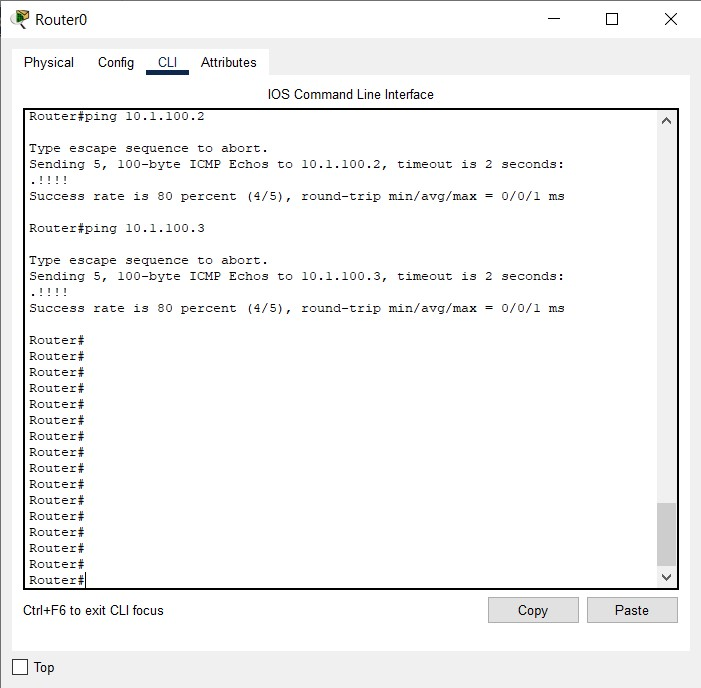
\includegraphics[width=0.75\textwidth]{figures/5.jpg}
    \caption{}
    \label{fig:fig1}
\end{figure}

\section{}%6
روترها نمی‌توانند اینترفیس‌های \lr{loopback} یکدیگر را پینگ کنند. چون رنج آن‌ها کاملا متفاوت است.
\begin{figure}[H]
    \centering
    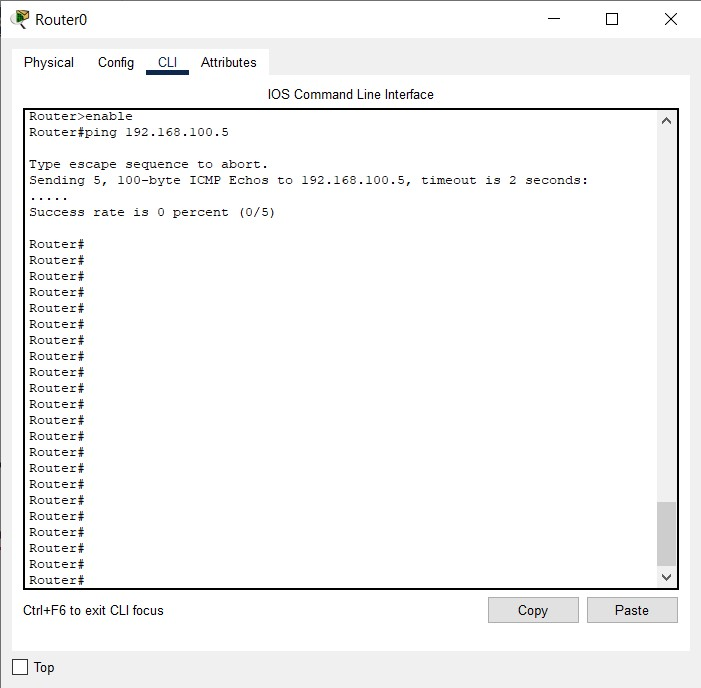
\includegraphics[width=0.75\textwidth]{figures/6.jpg}
    \caption{}
    \label{fig:fig1}
\end{figure}


\section{}%7
\begin{figure}[H]
    \centering
    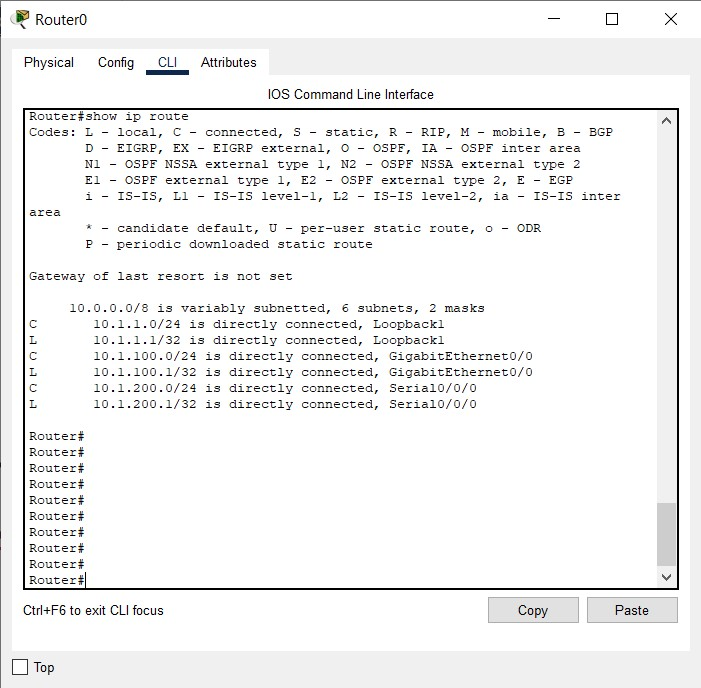
\includegraphics[width=0.75\textwidth]{figures/7.jpg}
    \caption{}
    \label{fig:fig1}
\end{figure}
\begin{figure}[H]
    \centering
    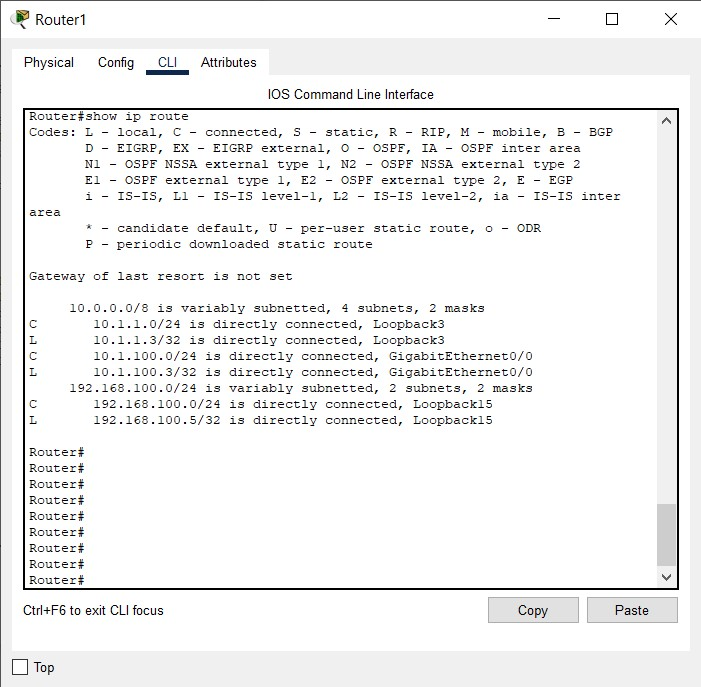
\includegraphics[width=0.75\textwidth]{figures/8.jpg}
    \caption{}
    \label{fig:fig1}
\end{figure}
\begin{figure}[H]
    \centering
    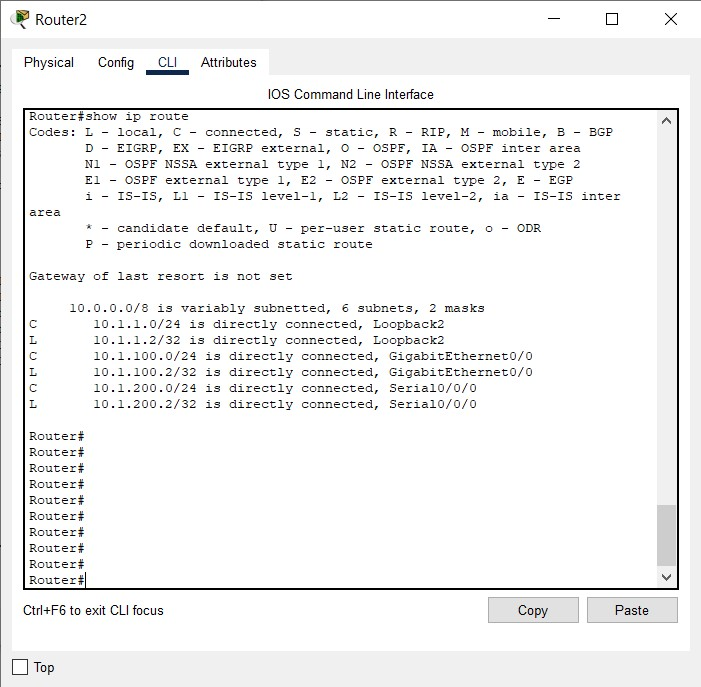
\includegraphics[width=0.75\textwidth]{figures/9.jpg}
    \caption{}
    \label{fig:fig1}
\end{figure}


\section{}%8
به طریق زیر پروتکل \lr{OSPF} را بر روی روتر پیکربندی می‌کنیم.
\begin{figure}[H]
    \centering
    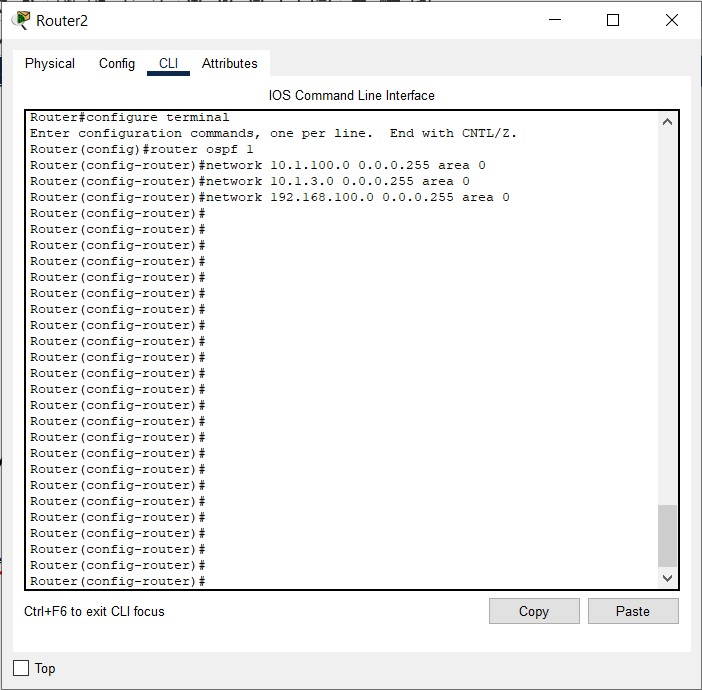
\includegraphics[width=0.75\textwidth]{figures/10.jpg}
    \caption{}
    \label{fig:fig1}
\end{figure}
\begin{figure}[H]
    \centering
    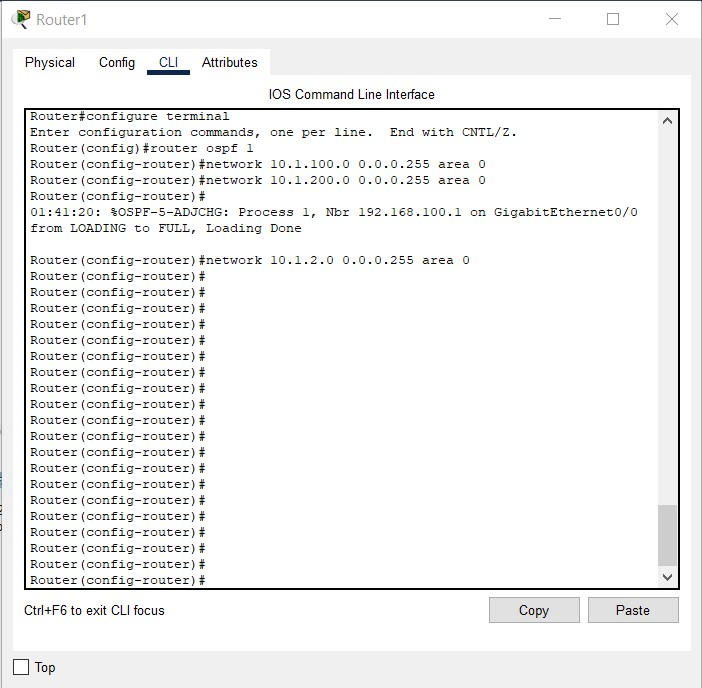
\includegraphics[width=0.75\textwidth]{figures/11.jpg}
    \caption{}
    \label{fig:fig1}
\end{figure}
\begin{figure}[H]
    \centering
    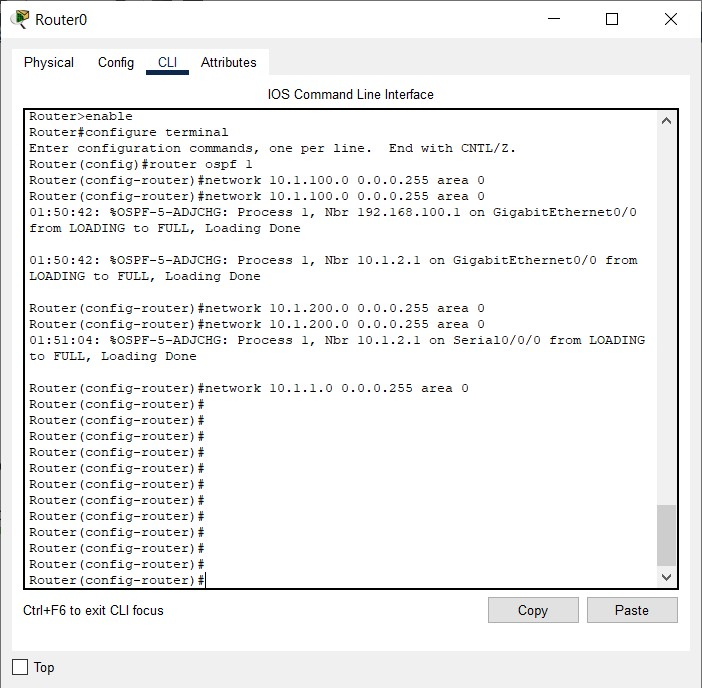
\includegraphics[width=0.75\textwidth]{figures/12.jpg}
    \caption{}
    \label{fig:fig1}
\end{figure}



\section{}%9

\begin{figure}[H]
    \centering
    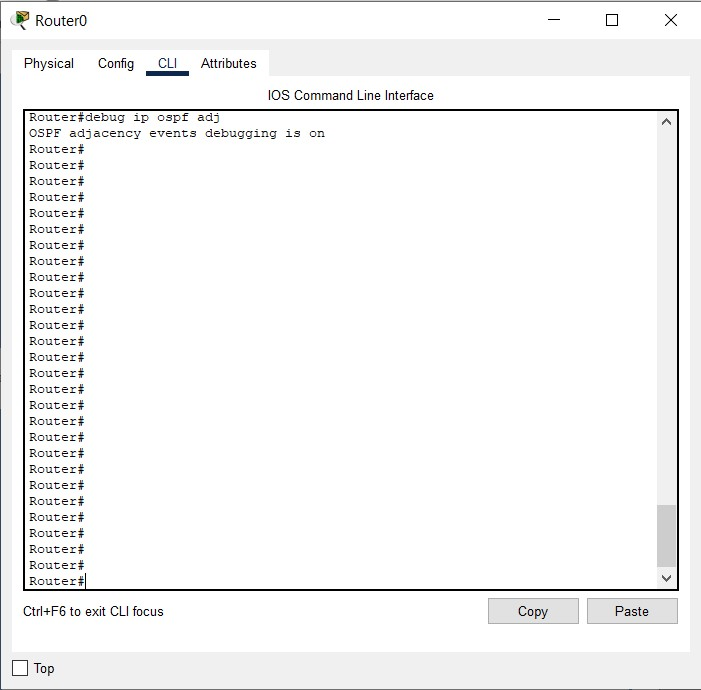
\includegraphics[width=0.75\textwidth]{figures/13.jpg}
    \caption{}
    \label{fig:fig1}
\end{figure}



\section{}%10
روترها به اینترفیس‌های \lr{loopback} یکدیگر نیز دسترسی دارند.
\begin{figure}[H]
    \centering
    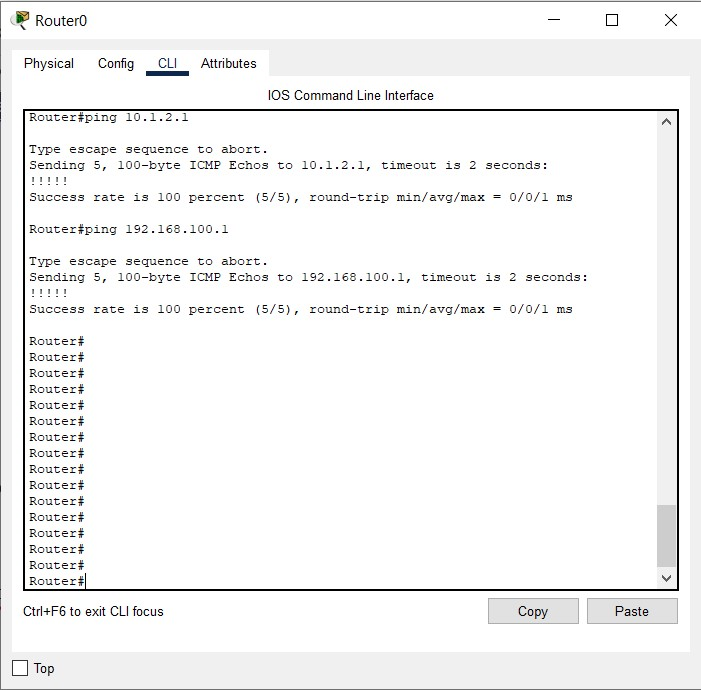
\includegraphics[width=0.75\textwidth]{figures/14.jpg}
    \caption{}
    \label{fig:fig1}
\end{figure}


\section{}%11
جدول مسیریابی روترها به شکل زیر است.
\begin{figure}[H]
    \centering
    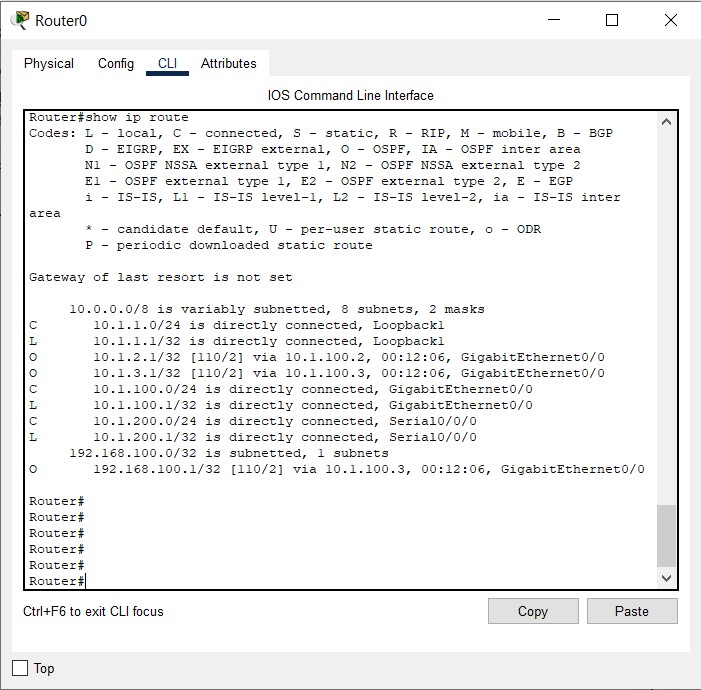
\includegraphics[width=0.75\textwidth]{figures/15.jpg}
    \caption{}
    \label{fig:fig1}
\end{figure}
\begin{figure}[H]
    \centering
    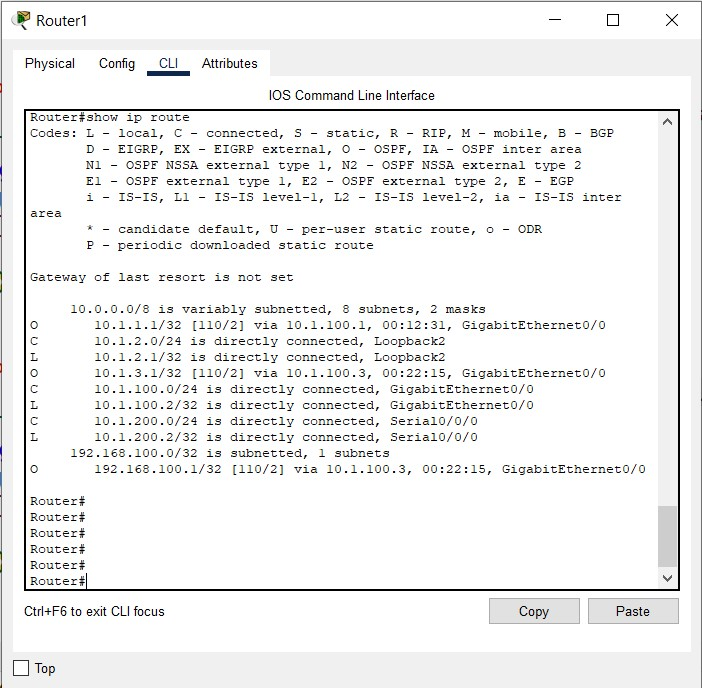
\includegraphics[width=0.75\textwidth]{figures/16.jpg}
    \caption{}
    \label{fig:fig1}
\end{figure}
\begin{figure}[H]
    \centering
    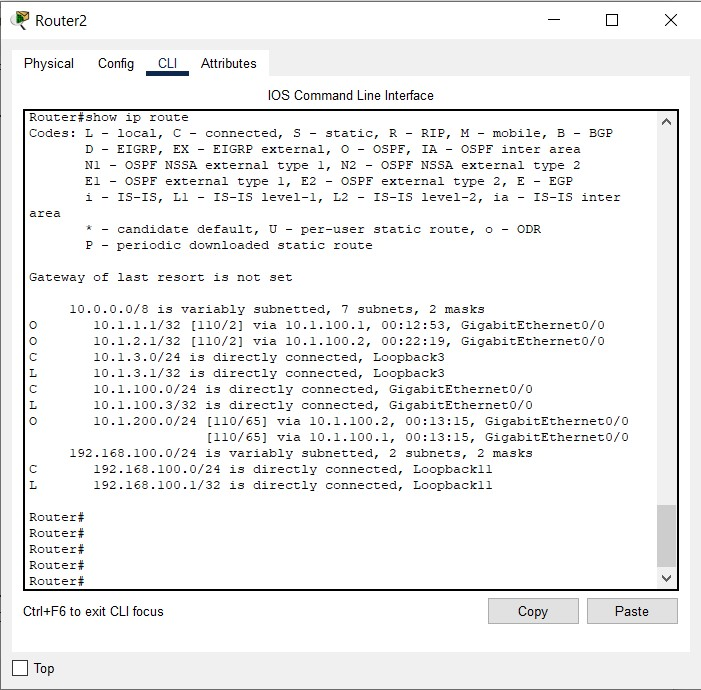
\includegraphics[width=0.75\textwidth]{figures/17.jpg}
    \caption{}
    \label{fig:fig1}
\end{figure}


\section{}%12
با دستور \lr{show ospf neighbor} می‌توان \lr{router id} را دید.
اگر دستی ست نشده باشد، آدرس آی‌پی \lr{loopback}ای که به روتر وصل است \lr{router id} است. اگر چند \lr{loopback} داشته باشد، آدرسی که بزرگ‌تر است.

\section{}%13
مسیریاب شماره‌ی 2 (سوم) \lr{DR} است.
\section{}%14
\begin{figure}[H]
    \centering
    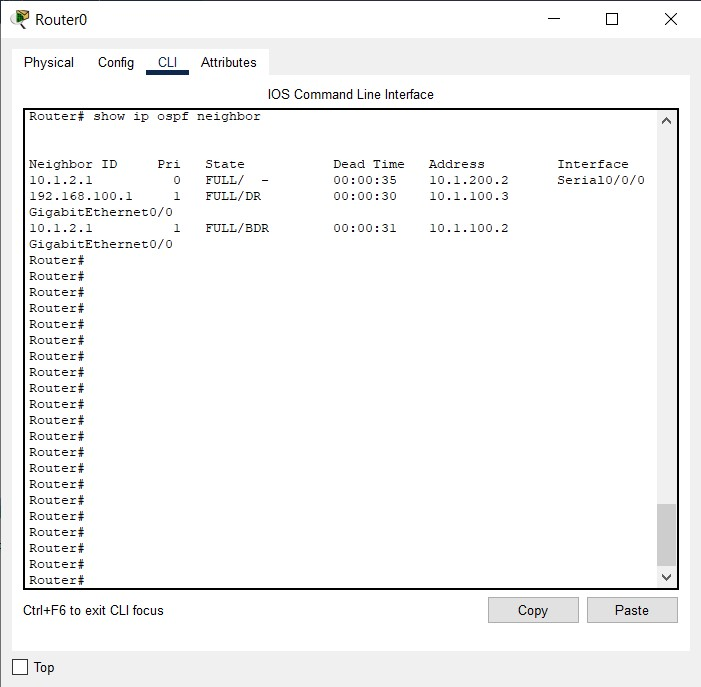
\includegraphics[width=0.75\textwidth]{figures/18.jpg}
    \caption{}
    \label{fig:fig1}
\end{figure}
\begin{figure}[H]
    \centering
    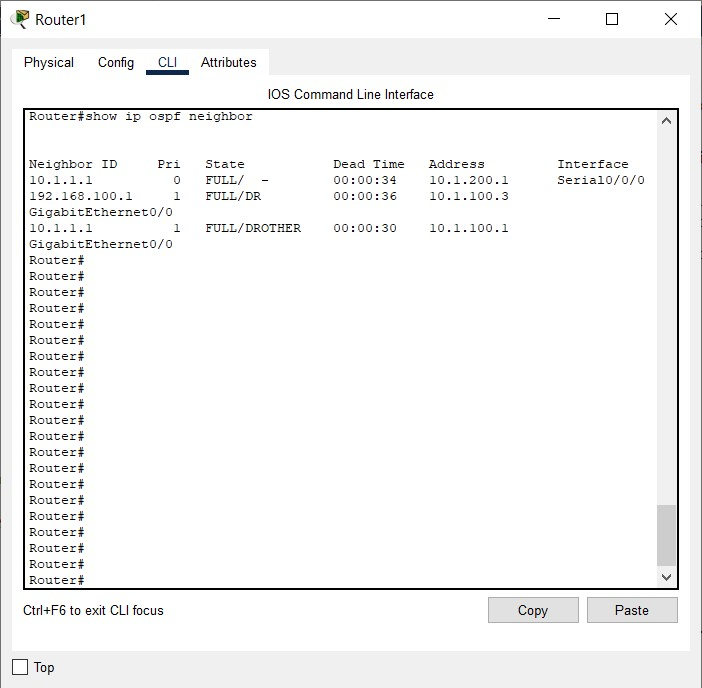
\includegraphics[width=0.75\textwidth]{figures/19.jpg}
    \caption{}
    \label{fig:fig1}
\end{figure}
\begin{figure}[H]
    \centering
    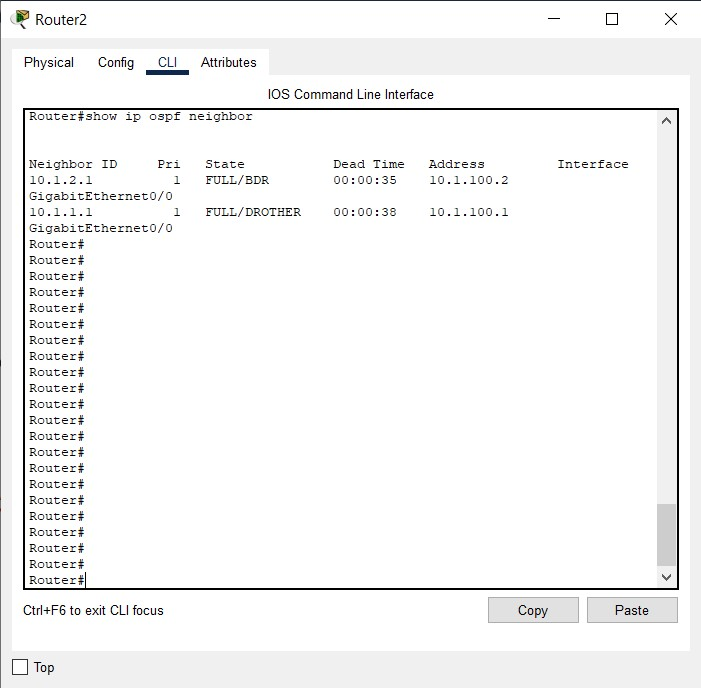
\includegraphics[width=0.75\textwidth]{figures/20.jpg}
    \caption{}
    \label{fig:fig1}
\end{figure}



\section{}%15

\begin{figure}[H]
    \centering
    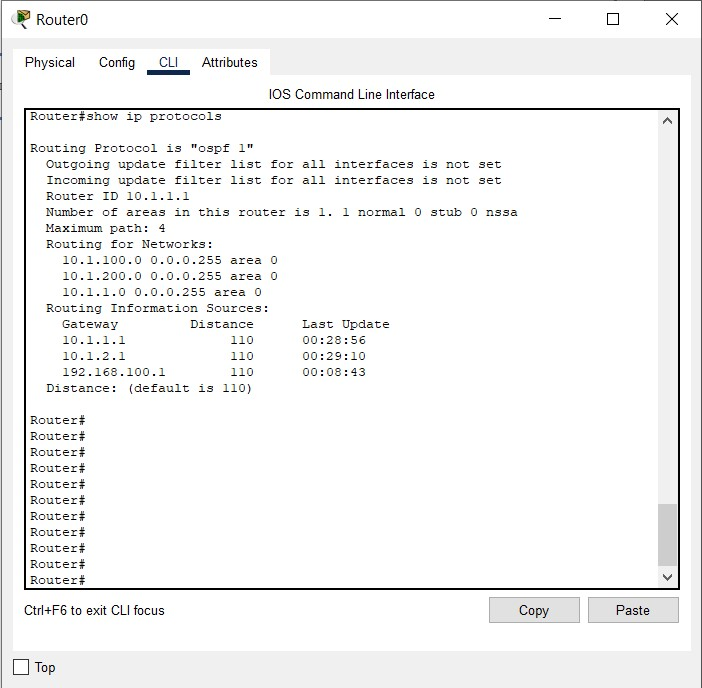
\includegraphics[width=0.75\textwidth]{figures/21.jpg}
    \caption{}
    \label{fig:fig1}
\end{figure}
\begin{figure}[H]
    \centering
    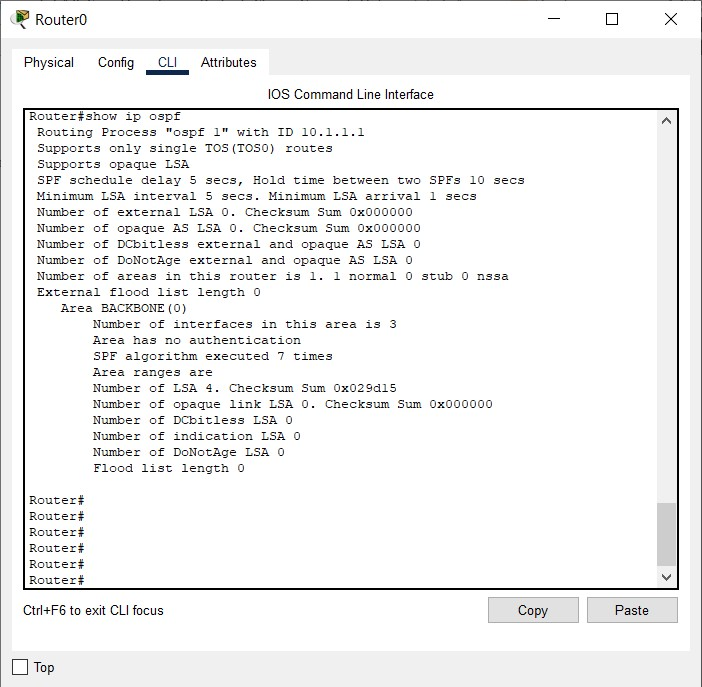
\includegraphics[width=0.75\textwidth]{figures/22.jpg}
    \caption{}
    \label{fig:fig1}
\end{figure}
\begin{figure}[H]
    \centering
    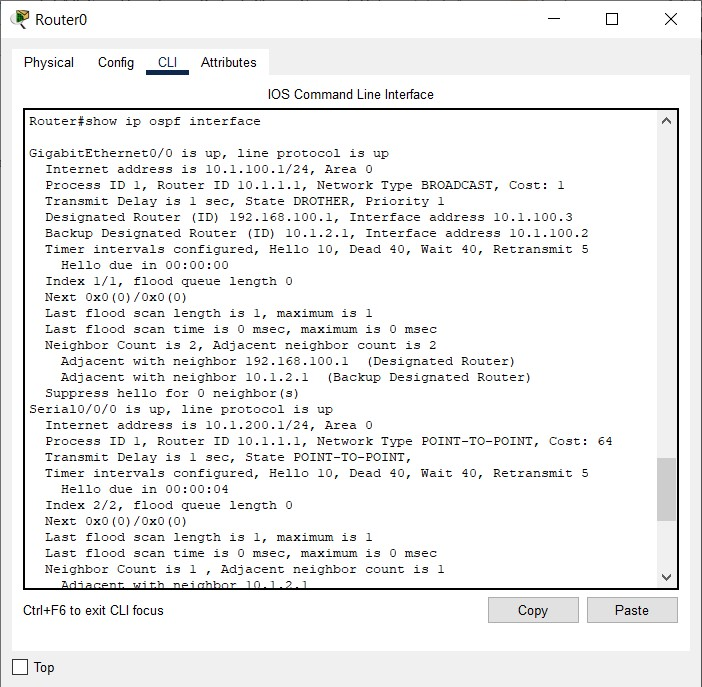
\includegraphics[width=0.75\textwidth]{figures/23.jpg}
    \caption{}
    \label{fig:fig1}
\end{figure}


\section{16 و 17}%16 17

\begin{figure}[H]
    \centering
    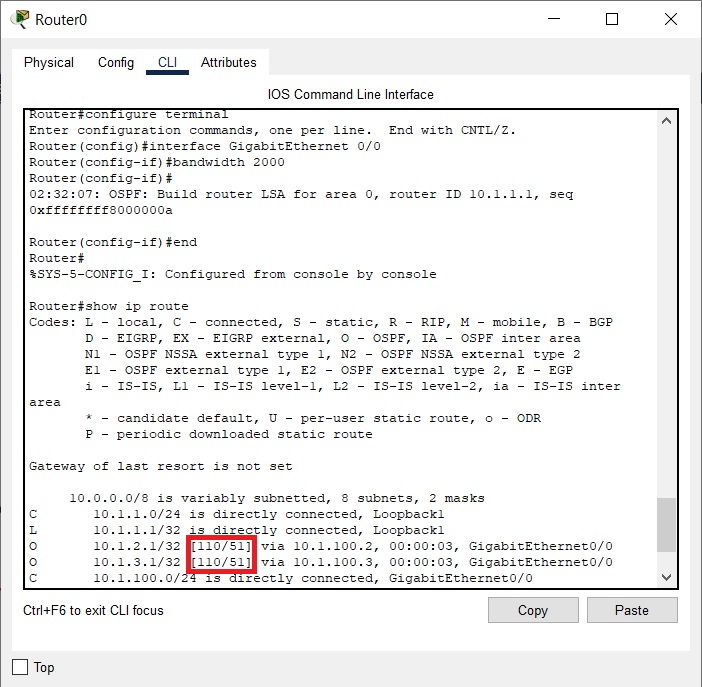
\includegraphics[width=0.75\textwidth]{figures/24.jpg}
    \caption{}
    \label{fig:fig1}
\end{figure}
\begin{figure}[H]
    \centering
    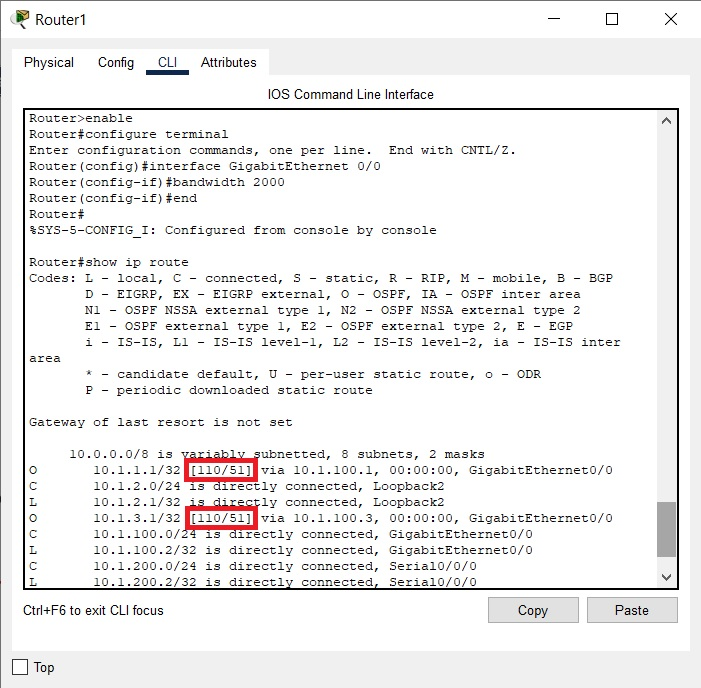
\includegraphics[width=0.75\textwidth]{figures/25.jpg}
    \caption{}
    \label{fig:fig1}
\end{figure}
\begin{figure}[H]
    \centering
    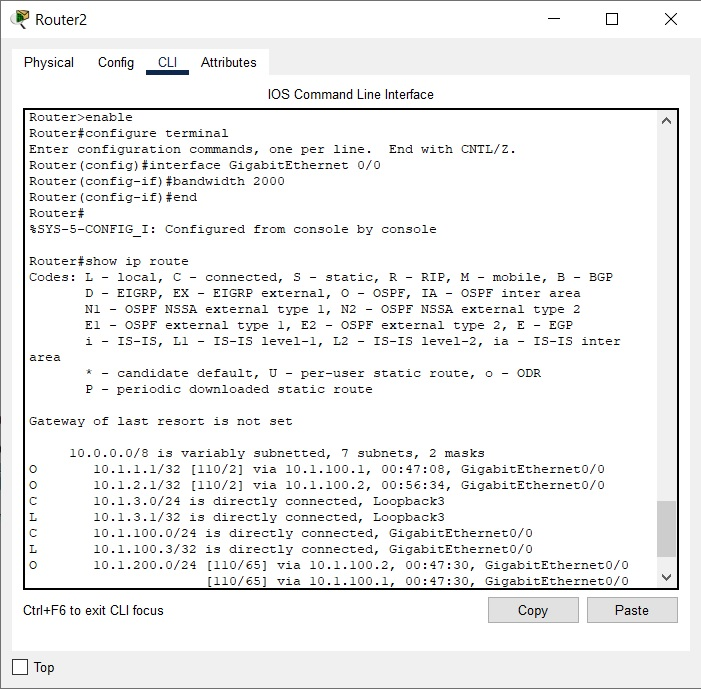
\includegraphics[width=0.75\textwidth]{figures/26.jpg}
    \caption{}
    \label{fig:fig1}
\end{figure}

\section{}%18
\begin{latin}
\VerbatimInput{source/x0.txt}
\end{latin}
\begin{latin}
\VerbatimInput{source/x1.txt}
\end{latin}
\begin{latin}
\VerbatimInput{source/x2.txt}
\end{latin}

%%%%%%%%%%%%%%%%%%%%%%%%%%%%%%%%%%%%%%%%%%%%%%

\section*{منابع}
\renewcommand{\section}[2]{}%
\begin{thebibliography}{99} % assumes less than 100 references
%چنانچه مرجع فارسی نیز داشته باشید باید دستور فوق را فعال کنید و مراجع فارسی خود را بعد از این دستور وارد کنید


\begin{LTRitems}

\resetlatinfont

\bibitem{b1}
\end{LTRitems}

\end{thebibliography}


\end{document}
